\chapter{Results}
\section{Users}
  In total, 15 people participated in the user study.
  They were recruited from MIT students,
  via dorm and living group mailing lists.

  All of the 15 people participated in the opening and closing interviews.
  However, only 8 of them participated in the Android portion of the study.
  The reasons for this will be discussed in the Section \ref{sec:Android}.

  The participants were compensated for their degree of participation,
  and the compensation structure is outlined in a table in Appendix A.

\section{Opening Questionnaire Results}
  The results from the opening questionnaire help to characterize the group's
  general thoughts on the subject of stress and support.
  
  Part of the survey included questions, scored on a Likert Scale,
  addressing to what degree they reach out to friends or family when troubled,
  and to what degree they feel supported by friends and family.
  The results are shown in Figure \ref{fig:likert}.

    \begin{figure}
    \centering
    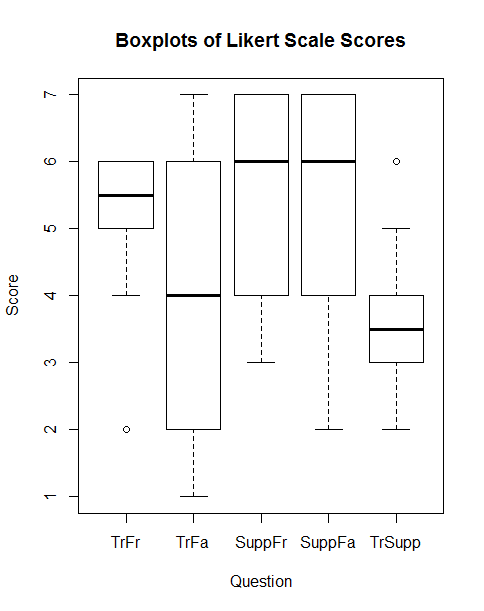
\includegraphics[width=0.6\textwidth]{likert.png}
    \caption{
      Results of Likert scale styled questions on the opening questionnaire.
      TrFa and TrFa asked whether participants want to talk to
      Friends or Family when Troubled.
      SuppFa and SuppFa asked whether participants felt supported by
      Friends or Family.
      TrSupp asked if they reached out, in general, when troubled.
    }
    \label{fig:likert}
    \end{figure}

  Also in the opening questionnaire, we administered a Perceived Stress Scale.
  The results, shown in a histogram in Figure \ref{fig:perceived_stress},
  show that in general, the users in this study had relatively low
  self-reported stress.

    \begin{figure}
    \centering
    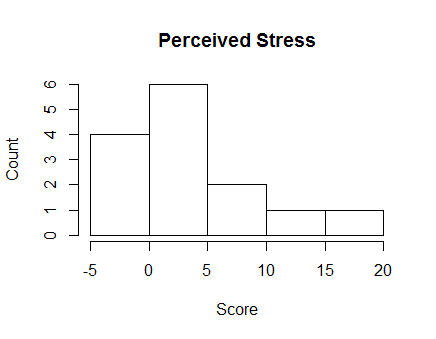
\includegraphics[width=0.6\textwidth]{perceived_stress.png}
    \caption{
      Distribution of Perceived Stress scores amongst the 15 participants.
    }
    \label{fig:perceived_stress}
    \end{figure}

\section{Opening Interview: Script Based Results}
  The opening interview, as mentioned in Section \ref{sec:opening_int},
  followed a script, so I'll briefly outline some of the
  prominent results from the 5 sections.

  \subsection{Support-Interest}
  Because the participants' situations were so different,
  the degree to which they wanted or needed social support were very different as well.
  On general degree of need and interest in reaching out,
  and high support-interest groups,
  support-interest defined as having a consistent desire and efforts to
  connect on an emotional and empathetic level with loved ones.
  To clarify, support-interest is a term I'll use when describing my participants,
  and is not a diagnostic term and definitely is not known to be
  correlated with other health and wellness outcomes.
  As far as I know, it is an indicator that becomes generally obvious
  on interview with the participants,
  and only represents the current situation of the interviewee, in snapshot.

  On the low support-interest end, two interviewees seemed especially independent,
  expressing a desire for and general pattern of dealing with things
  themselves, without much external input,
  and preference for keeping their concerns to themselves.
  They were by no means not social,
  both reported having plenty of friends that they interacted with regularly,
  but they chose to keep them at a greater distance when it came to things
  they were particularly sensitive about.
  When asked
  about how they discuss serious subjects with those closest to them,
  they tend to express a lack of interest.
  A quote from one of them, Participant 1847,
  on her thoughts about keeping her privacy,
  helps to express the sentiment:
  \textit{
  ``[These thoughts are] my personal complications.
  I usually don't share that much with people because
  I'm not comfortable with them knowing me too well.
  I prefer to keep a personal boundary."
  }

  On the high support-interest end, there was a lot of variability.
  High support-interest people included my married interviewees, who notably,
  married within the last 5 years or so,
  and expressed being very open with their spouses, sharing everything.
  They also included a participant very active in her church community,
  and other individuals close with their parents or significant others.
  These participants expressed spending a lot of time invested in
  sharing feelings and struggles.
  Quotes associated with them included:
  \begin{itemize}
  \item \textit{
  ``She was the first person that I felt like I could talk freely with.
  We can talk about anything and everything.
  She asks questions that really pin at trying to figure out
  where emotions are coming from, what's really bothering me at a certain time.
  Just the fact that she lets me talk freely and with understanding
  makes me more comfortable."
  }
  - Participant 8594, about her mentor figure.
  \item \textit{
  ``I talk most to my mom... I try to tell my mom everything.
  She's not pushy, but she won't let me not tell her things.
  She'll ask `And then what did the the doctor say? And then?
  Whats this medicine? I need to look it up!'
  [So] then I tell her everything, because she worries."
  }
  - Participant 1496, about her mother.
  \item  \textit{
  ``We're on GChat a lot.
  We chat throughout the day.
  I know how she's feeling with about a 15 minute resolution."
  }
  - Participant 3792, about his girlfriend.
  \item \textit{
  ``I have a really honest relationship with [boyfriend name].
  He'll be the first one to check in after a medical appointment,
  so is most aware...
  Rather than him trying to make sense of it,
  it makes more sense for him to just be supportive and be there.
  ... If I say anything negative, he'll jump on it.
  If I'm feeling down on myself,
  just him kinda being, `hey, you're doing the best you can.'
  ... Sometimes I'm in the place to hear it."
  }
  - Participant 4416, about her boyfriend.
  \item \textit{
  ``I have a group of two women.. we call ourselves accountability partners.
  We meet up, like, every week.
  The idea of keeping each other accountable is
  [about] committing to listen to one another, encourage one another,
  and challenge one another to live a life of faith."
  }
  - Participant 5397, about her certain members of her church community.
  \end{itemize}

  \subsection{Choosing People and Choosing Topics}
  On discussing the support network of the interviewees,
  they tended to have a certain group of people that they turned to for
  general day-to-day support.
  These people could be family, or family-like people, as well as friends,
  but most times, participants had a strong preference towards one or the other.

  In most cases, the interviewee chose to discuss serious subjects,
  about things that were really on their minds,
  with only friends or only family,
  and chose to discuss only mundane, less serious topics with the other.
  For example, Participant 1010, talking about her parents,
  expressed a common sentiment.
  \textit{
  ``We only talk about mundane things...
  things not directly related to life."
  }

  \subsection{Serious Situation}
  Although the call for participant recruitment called for participants
  dealing with some serious situation in their lives,
  whether mourning or illness or other unusual difficulty of transition,
  the severity of the participants' situations varied.

  On the lighter end of the spectrum included six participants who were
  dealing with regular academic and career pressures.
  On the heavier end,
  three participants were dealing with very serious chronic illnesses,
  another was bereaved, and other were battling some daunting transitions.

  \subsection{Meeting Needs}
  Luckily, all of my participants who wanted support had people
  who could provide it.
  However, as anticipated by other research \cite{skeels10},
  when the needs grew, it became harder for some of my participants to get
  what they needed.

  Participant 9541 expressed a general sentiment about discussing tough topics:
  \textit{
  ``Feeling like you need it and actually reaching out are two different things.
  It's a lot harder to say `I'm struggling with whatever's going on.'"
  } and Participant 
  ``A year ago, I was not very good about reaching out to people.
  We didn't really reach out to people for help.
  It takes a lot of energy to reach out to people and explain what's going on.
  [We thought]
  `If these people are really my friends, they should be reaching out to me,'
  but actually, if they don't know, they don't know.
  Nowadays, there's a group of people we'll email or call.
  Maybe we should be asking a few people, specifically, to be on-call."

  \subsection{Technology}
  On technology,
  my participants tended to be technically savvy.
  This is likely due to the age range of the participants,
  the youngest of which was 18, and the oldest 30.
  Consistent with previous research,
  they used a complex range of technologies to connect
  with friends and family near and at distance,
  for a range of complicated reasons.
  More convenient forms of communication,
  such as text or other forms of instance message,
  were used frequently for casual things and keeping in touch,
  and other modes of communication, such as video, phone, or in person meetings,
  were used for more serious topics.
  The exception to this was email,
  which despite being digital and text based, 
  afforded a level of thoughtfulness that participants
  felt were especially valuable.
  One participant found emails the best medium for reconnecting
  with distant friends on the nature and current condition of her
  chronic illness,
  and another participant who had depressive episodes found that
  email communications fell better into her comfort zone during the dark times.

\section{Opening Interview: Other Trends}
  The trends addressed by the script of the opening interview touched on
  some important topics, but the most interesting results
  were other patterns and phenomena
  that were not anticipated by the script.

  \subsection{Direction of Awareness}
  In many cases, there was a clear directionality to the type of awareness
  information shared.
  One recurrent example was with parents,
  when the daughter or son tends to report a lot to the parent,
  and the parent reports relatively little in return.
  Other relationships, such as between siblings or friends,
  can also be very directional,
  with one party in the habit of disclosing more to the other.
  for example, Participant 1010 explained her relationships:
  \textit{
  ``With some of my friends, I like to know what they're doing.
  I kinda mother them.
  I like to make sure they're doing okay."
  }

  \subsection{Extreme Information Withholding}
  Another phenomenon that became apparent with interviews is that
  many, even normally trusting, close relationships,
  can incorporate extreme instances of information withholding.
  One relatively whimsical example was brought up
  when the topic of awareness and updates from family was brought up.
  \textit{
    ``
    They don't tell me anything. No.
    They feel like I should focus on me.
    Even when my dog passed away, they didn't tell me for an entire month.
    They didn't want me to be upset.
    I just noticed the dog wasn't there, and they never straight up told me."
  } - Participant 2928

  It's important to note that the story is one instance of a general
  trend of not sharing bad news.
  This can be as simple as preferring to look on the bright side:
  \textit{
  ``I try to look on the bright side.
  For example, my Facebook page used to be full of sad things.
  I decided not to do that anymore."
  } - Participant 3792
  or \textit{
  ``[My struggles are] not really fun to talk about.
  Most people already have enough on their plate"
  }
  - Participant 9451
  
  This can also be taken to the extreme.
  One specific example from my participants involved
  completely not telling family members about a serious issue,
  while maintaining communications otherwise.

  \subsection{Changes in Support Structure}
  Lastly, closely related to the extreme information withholding,
  there are many situations in our lives that result in
  drastic changes in the nature of our support structure.
  The drastic changes that I observed in interviews
  tended to involve a falling out of some sort.
  These could be between family members,
  significant others, or even friends.
  Another notable cause for a drastic change in support structure,
  if less common and much more tragic: death.
  When the person who passed away had a pivotal role in the support
  structure of another, it can be even harder to cope with
  the difficult period of mourning.

\section{Android}
\label{sec:Android}

\section{Data and Questions to Answer}

  Using server data:
  \begin{enumerate}
    \item When are topics made?
    \item How many topics per week?
    \item How many messages per week?
    \item Who receives topics?
    \item How long does a topic live?
  \end{enumerate}

  Using Google Analytics App data:
  \begin{enumerate}
    \item How much time is spent on the app?
    \item How much of that is with individual plants/writing notes?
    \item What time of day is the app accessed?
    \item For browsing vs status updating?
  \end{enumerate}
